\section{Aproksymacja jednostajna}
%%%%%%%%%%%%%%%%%%%
\begin{frame}{Aproksymacja jednostajna}
	Dla $F(x)$ określonej na $[a,b]$ szukamy $f(x)$:
	 $$min ||F(x)-f(x)|| = min\underbrace{sup_{x \in [a,b]}|F(x)-f(x)|}_{\text{norma Czebyszewa}}$$
\end{frame}
%%%%%%%%%%%%%%%%%%%
\begin{frame}
	\begin{block}{Twierdzenie Weierstrassa}
	Jeżeli $F(x) \in C^0[a,b]$, to dla każdego $\varepsilon>0$ można dobrać $n(\varepsilon)$ takie, że istnieje $W_n(x): |F(x)-W_n(x)|<\varepsilon$ \newline
    \newline Wniosek: $F(x)$ można aproksymować jednostajnie wielomianami.
	\end{block}
    Szukamy $a_i$:\newline
    $W_n(x) = \sum_{i=0}^{n}a_ix^i$ aby $min E_n$, \newline
    $E_n = max_{x \in [a,b]} |F(x) - W_n(x)|$
\end{frame}
%%%%%%%%%%%%%%%%%%%
\begin{frame}
	\begin{block}{Twierdzenie Borela}
		Jeśli $F(x)\in C^0[a,b], n$ - naturalna, to istnieje $W_n(x)$ będący najlepszym przybliżeniem $F(x)$.
	\end{block}
    \begin{block}{Twierdzenie Czebyszewa}
    	Wielomian $W_n(x)$ będący najlepszym przybliżeniem $F(x)$ jest tylko jeden.
    \end{block}
\end{frame}
%%%%%%%%%%%%%%%%%%%
\begin{frame}{Metoda szeregów potęgowych - szereg Taylora}
Prostą metodą aproksymacji jednostajnej jest metoda szeregów potęgowych t.j. używamy pierwszych n+1 wyrazów szeregu Taylora:
	$$W_n(x) = \sum_{k=0}^{n}\frac{F^{(k)}(x_0)}{k!}(x-x_0)^k$$
    oszacowanie błędu aproksymacji $\rightarrow$ reszta Lagrange'a:
    $$F(x)-W_n(x) = \frac{F^{n+1}(\eta)}{(n+1)!}(x-x_0)^{n+1},\eta \in [a,b]$$
\end{frame}
%%%%%%%%%%%%%%%%%%%
\begin{frame}{Przybliżenia Padé}
	\textbf{ang.} Padé approximation, rational function approximation \newline
    \newline
    Aproksymujemy funkcję $F(x)$ za pomocą funkcji wymiernej $r(x)$.
    \newline
    Funkcja wymierna $r(x)$ stopnia $N = n+m$ ma postać:
    $$r(x) = \frac{p(x)}{q(x)} = \frac{p_0+p_1x+\ldots+p_nx^n}{q_0+q_1x+\ldots+q_mx^m}$$
    \begin{itemize}
    \item nieredukowalna (p, q - są względnie pierwsze - nie mają wspólnych dzielników)
    \item określona w $x=0\Rightarrow q_0 \not = 0, \Rightarrow q_0=1$ (zwykle)
    \item do określenia $N+1 = n+m+1$ współczynników
    \end{itemize}
\end{frame}
%%%%%%%%%%%%%%%%%%%
\begin{frame}{Technika aproksymacji Padé}
	Jest to sposób określenia $\{p_i,q_j\}, i = 0,..,n,j = 0,..,m$ przy zadanych $n,m$ 
    $$F(x) - r(x) = F(x) - \frac{p(x)}{q(x)}=\frac{F(x) \cdot q(x) - p(x)}{q(x)}$$
    Niech $F(x) = \sum_{i=0}^{\infty}a_i \cdot x^i \rightarrow$ szereg Maclaurina
    $$F(x) - r(x) = \frac{\sum_{i=0}^{\infty}a_ix^i \cdot \sum_{i=0}^{m}q_ix^i - \sum_{i=0}^{n}p_ix^i}{q(x)}$$
    Należy dobrać $p_0,p_1,..,p_n$ i $q_1,..,q_m$ tak, aby  rozwinięcia $F(x)$ i $r(x)$ w szereg Maclaurina były jak najbardziej zgodne czyli możliwie najwięcej pochodnych $F(x)$ i $r(x)$ w $x=0$ było równych:
    $$F^{(k)}(0)-r^{(k)}(0) = 0, k=0,1,..,N$$
    
\end{frame}
\begin{frame}{}
$$w(x)=ax^3+bx^2+cx+d \text{, } w(0)=d \text{ i } w(0)=0 \rightarrow d=0$$ 
$$w'(x)=3ax^2+2bx+c  \text{, } w'(0)=c \text{ i } w'(0)=0 \rightarrow c=0$$
$$w''(x)=6ax+2b  \text{, } w''(0)=2b  \text{ i } w''(0)=0 \rightarrow b=0$$
$$w'''(x)=6a  \text{, } w'''(0)=6a \text{ i } w'''(0)=0 \rightarrow a=0$$
\end{frame}
%%%%%%%%%%%%%%%%%%%
\begin{frame}
    To znaczy, że licznik:
    $$(a_0+a_1x+..)(1+q_1x+..+q_mx^m)-(p_0+p_1x+..+p_nx^n)$$
    nie powinien mieć wyrazów stopnia $\leqslant N$. Dla uproszczenia zapisu:
    \begin{center}
    	$p_{n+1} = p_{n+2}=..=p_N=0$ i $q_{m+1} = q_{m+2} = .. =q_N = 0$
    \end{center}
    Wtedy współczynniki: $\sum_{i=0}^{k}a_iq_{k-i}-p_k$ powinny być równe $0$, a znalezienie $p(x)$ i $q(x)$ polega na rozwiązaniu układu równań liniowych:
    $$\sum_{i=0}^{k}a_iq_{k-i}-p_k = 0; k=0,1,...,N$$
\end{frame}
\begin{frame}
    \begin{figure}
        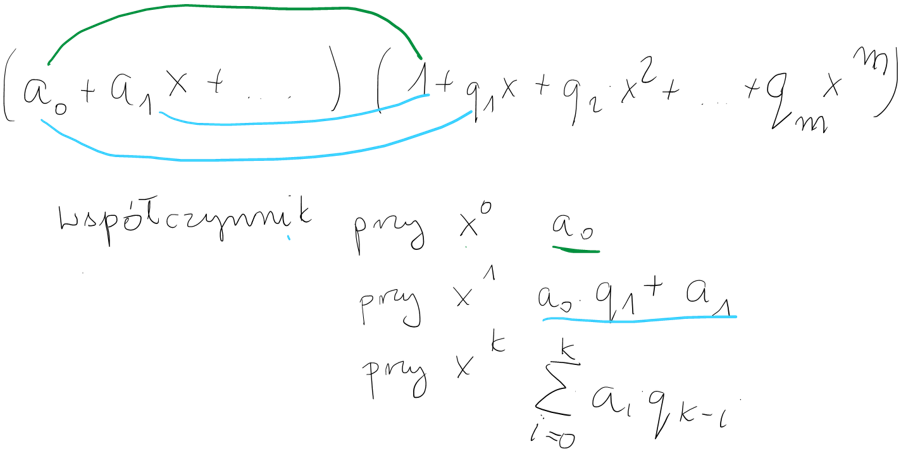
\includegraphics[height=0.6\textheight]{img/5/pade1.png}
    \end{figure}
\end{frame}
%%%%%%%%%%%%%%%%%%%
\begin{frame}{Typowy przykład}
	$$ F(x) = \big[7+(1+x)^{\frac{4}{3}}\big]^{\frac{1}{3}} \approx 2+\frac{1}{9}x+\frac{1}{81}x^2-\frac{49}{8748}x^3+\frac{175}{78732}x^4+\ldots $$
    \begin{block}{Uwagi}
    	\begin{itemize}
        \item w praktyce: $N = n+m$ - ustalone: $\left\{\begin{array}{ccl}
        	n & = & m \\
            n & = & m+1
        \end{array}\right.$
    	\end{itemize}
    \end{block}
\end{frame}
%%%%%%%%%%%%%%%%%%%
\begin{frame}
    \begin{figure}
        \includegraphics[height=0.8\textheight]{img/5/pade.png}
    \end{figure}
\end{frame}